\section{Analysis}

\subsection{Use Case analysis}

\subsubsection{Class Candidates}
In order to find potential class candidates, every noun of the detailed Use
Cases are found. These are potential candidates, and can be sorted to avoid
duplicates and candidates that won’t be turned into classes. Naturally, every
potential class for the entire system will not be found, as this only reflects
use cases. A potential class candidate such as MES (where Start and Stop
functionality would otherwise be implemented) will not be reduced to a single
class and is therefore not added to the list of class candidates.

The final list of classes, as well as a description of them, can be seen in
table \ref{table:class_candidates}.

\begin{table}[ht]
    \begin{tabularx}{\textwidth}{|>{\RaggedRight}p{4cm}|>{\RaggedRight}p{6cm}|>{\RaggedRight}X|}
    \hline
    \textbf{Class Candidate} & \textbf{Attributes}                                                                                                     & \textbf{Definition}                                                                    \\ \hline
    Batch                    & Id, type, product\_amount (total, defect, acceptable), amount (time), state (current, history), OEE, production\_speed, & A batch refers to a specific batch of products the brewery has made                    \\ \hline
    Product                  & Id, type, Ingredients,                                                                                                  & Product refers to the different options of beer to be produced                         \\ \hline
    Ingredient               & Name, id                                                                                                                & An ingredient refers to a specific ingredient. Products contain a list of ingredients. \\ \hline
    \end{tabularx}
    \caption{Potential class candidates}
    \label{table:class_candidates}
    \end{table}

\subsubsection{UML Analysis Diagram}
From the verb/noun analysis from the previous chapter, the UML analysis diagram
seen in figure \ref{figure:analysis_diagram}, can be generated. This diagram
shows the classes and attributes found in the requirements from the project
description.

\begin{figure}[ht]
	\centering 
	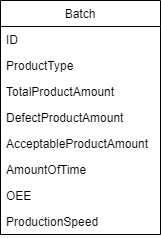
\includegraphics[scale=0.6]{images/diagrams/UML_Analysis_Diagram.drawio.png}
	\caption{UML Analysis diagram}
	\label{figure:analysis_diagram} 
\end{figure}

\subsection{Use Case Realisation}

\subsubsection{Sequence Diagrams}
A sequence diagram shows the system events for a given scenario of a use case,
and how the actor interacts with the system to solve the use case. There are two
kinds of sequence diagrams, system and operation. The system sequence diagram
displays the system as a 'black box', where the internal system events are not
shown, but only the external. This means that the diagram displays how actors
generate system events and what the system output is. Furthermore, the diagram
functions as a timeline for the system events. \\

\myworries{maybe add a system sequence diagram and explain why we used it}

The operation sequence diagram displays the system as a 'white box', where both
the internal and external system events are described, as seen in figure
\ref{figure:sequence_diagram}.

\begin{figure}[H]
\centering 
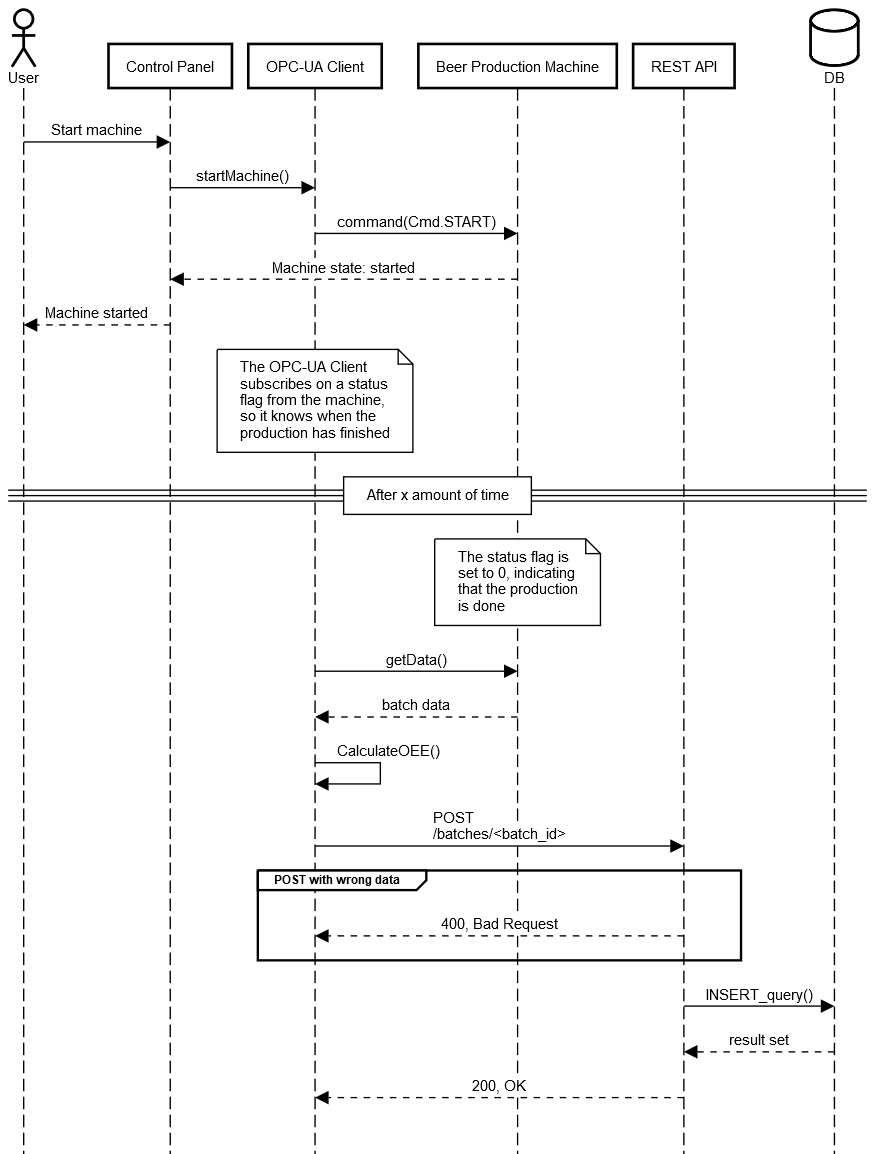
\includegraphics[scale=0.3]{images/sequence_operation/start.png}
\caption{Sequence diagram: start}
\label{figure:sequence_diagram} 
\end{figure}

This sequence diagram is used to identify system functions, as the events shown
in the diagram are the functions needed to complete the use case. In this
specific use case, the actor, the user, wants to start the beer production
machine. The user interacts with the control panel by pressing the start button,
which then sends a command to the OPC-UA client. The OPC-UA client interprets
the command as a start machine command, which triggers an event in the OPC-UA
client to send a command to the beer production machine. The beer production
machine interprets the command as a start command, which then turns on the 
machine. As a response to the user, to beer production machine sets a flag
which the control panel reacts to, and sends a message to the user. \\

When the beer production has finished, the OPC-UA client collects all relevant
data from the beer production machine. This data is used to calculate the
optimal production speed, estimate the error function, and calculate the OEE.
These calculations are used to optimise the beer production. The calculated data
and the data collected from the machine is then stored in a database. This
happens through a REST API which acts as a translator between the different 
subsystems within the MES.

            % \begin{enumerate}
            %     \item A beer type should be selected
            % \end{enumerate}

\subsubsection{Operation Contracts}
An operation contract describes the responsibility of the operation. 
The contract focuses on what the operation can change, and not how it is changed. 
It is also used to describes the state of the system before and after the 
operation is called.
\begin{table}[H]
    \begin{tabularx}{\textwidth}{|>{\RaggedRight}p{3.7cm}|>{\RaggedRight}X|}
        \hline
        \multicolumn{2}{|c|}{\textbf{start}}\\
        \hline
        \textbf{System operation} & start\\
        \hline
        \textbf{Cross References} & Use case: Start machine see table \ref{table:usecase_start} \\
        \hline
        \textbf{Responsibility} & Starting the beer machine if the pre-conditions 
        is met.
            If the pre-conditions is not met, the beer machine will not start \\
        \hline
        \textbf{Output} & The beer machine started the production\\
        \hline
        \textbf{Pre-conditions} & 
            The beer production machine needs to be in
            ready mode, that is, not producing beer. \\
        \hline
        \textbf{Post-conditions} & The beer machine started brewing\\
        \hline
    \end{tabularx}
    \caption{Operation Contracts start} 
    \label{table:Operation_Contracts_start}
\end{table}

\begin{table}[H]
    \begin{tabularx}{\textwidth}{|>{\RaggedRight}p{3.7cm}|>{\RaggedRight}X|}
        \hline
        \multicolumn{2}{|c|}{\textbf{stopProduction}}\\
        \hline
        \textbf{System operation} & stopProduction\\
        \hline
        \textbf{Cross References} & Use case: Stop the beer Machine see table \ref{table:usecase_stop}\\
        \hline
        \textbf{Responsibility} & Stop's the beer machine if the pre-conditions is met.
        If the pre-conditions is not met, the beer machine will not do anything\\
        \hline
        \textbf{Output} & The beer machine is stopped\\
        \hline
        \textbf{Pre-conditions} & The beer machine needs to be running\\
        \hline
        \textbf{Post-conditions} & The beer machine is stopped\\
        \hline
    \end{tabularx}
    \caption{Operation Contracts stopProduction} 
    \label{table:Operation_Contracts_stopProduction}
\end{table}


\begin{table}[H]
    \begin{tabularx}{\textwidth}{|>{\RaggedRight}p{3.7cm}|>{\RaggedRight}X|}
        \hline
        \multicolumn{2}{|c|}{\textbf{reset}}\\
        \hline
        \textbf{System operation} & reset \\
        \hline
        \textbf{Cross References} & Use case: reset see table \ref{table:usecase_reset} \\
        \hline
        \textbf{Responsibility} & It is responsible for resetting the beer 
                machine.\\
        \hline
        \textbf{Output} & reset the beer machine. \\
        \hline
        \textbf{Pre-conditions} & The beer production machine needs to be in
                ready mode, that is, not producing beer. \\
        \hline
        \textbf{Post-conditions} & The beer production machine has been reset. \\
        \hline
    \end{tabularx}
    \caption{Operation Contracts reset} 
    \label{table:Operation_Contracts_reset}
\end{table}

\begin{table}[H]
    \begin{tabularx}{\textwidth}{|>{\RaggedRight}p{3.7cm}|>{\RaggedRight}X|}
        \hline
        \multicolumn{2}{|c|}{\textbf{clear}}\\
        \hline
        \textbf{System operation} & clear\\
        \hline
        \textbf{Cross References} & Use case: clear see table \ref{table:usecase_reset} \\
        \hline
        \textbf{Responsibility} & It is responsible for clearing the beer 
                machine. \\
        \hline
        \textbf{Output} & The beer machine has been cleared. \\
        \hline
        \textbf{Pre-conditions} & The beer production machine needs to be in
                ready mode, that is, not producing beer. \\
        \hline
        \textbf{Post-conditions} & The beer production machine has been cleared.\\
        \hline
    \end{tabularx}
    \caption{Operation Contracts clear} 
    \label{table:Operation_Contracts_clear}
\end{table}

\begin{table}[H]
    \begin{tabularx}{\textwidth}{|>{\RaggedRight}p{3.7cm}|>{\RaggedRight}X|}
        \hline
        \multicolumn{2}{|c|}{\textbf{display live data}}\\
        \hline
        \textbf{System operation} & displayLiveData\\
        \hline
        \textbf{Cross References} & Use case: displayLiveData see table \ref{table:usecase_displayLiveData} \\
        \hline
        \textbf{Responsibility} & It is responsible for posting data to the client. \\ 
        \hline
        \textbf{Output} & Post data to the client.  \\
        \hline
        \textbf{Pre-conditions} & The beer production machine needs to be on and
                producing beer. \\
        \hline
        \textbf{Post-conditions} & Live data has been displayed for the user. \\
        \hline
    \end{tabularx}
    \caption{Operation Contracts monitorAndDisplayData} 
    \label{table:Operation_Contracts_monitorAndDisplayData}
\end{table}

\begin{table}[H]
    \begin{tabularx}{\textwidth}{|>{\RaggedRight}p{3.7cm}|>{\RaggedRight}X|}
        \hline
        \multicolumn{2}{|c|}{\textbf{batchReport}}\\
        \hline
        \textbf{System operation} & batchReport\\
        \hline
        \textbf{Cross References} & Use case: batchReport see table \ref{table:usecase_batchReport} \\
        \hline
        \textbf{Responsibility} &  Make a report after the pre-conditions is met
                and adds the report to the database.\\
        \hline
        \textbf{Output} & Produces a batch report and display it for the user.\\
        \hline
        \textbf{Pre-conditions} & The beer Machine needs to have produced a batch.\\
        \hline
        \textbf{Post-conditions} & A batch report has been displayed for the
                user. \\
        \hline
    \end{tabularx}
    \caption{Operation Contracts produceBatchReport} 
    \label{table:Operation_Contracts_produceBatchReport}
\end{table}

\subsubsection{Updated UML Class Diagram}
\begin{figure}[ht]
\centering 
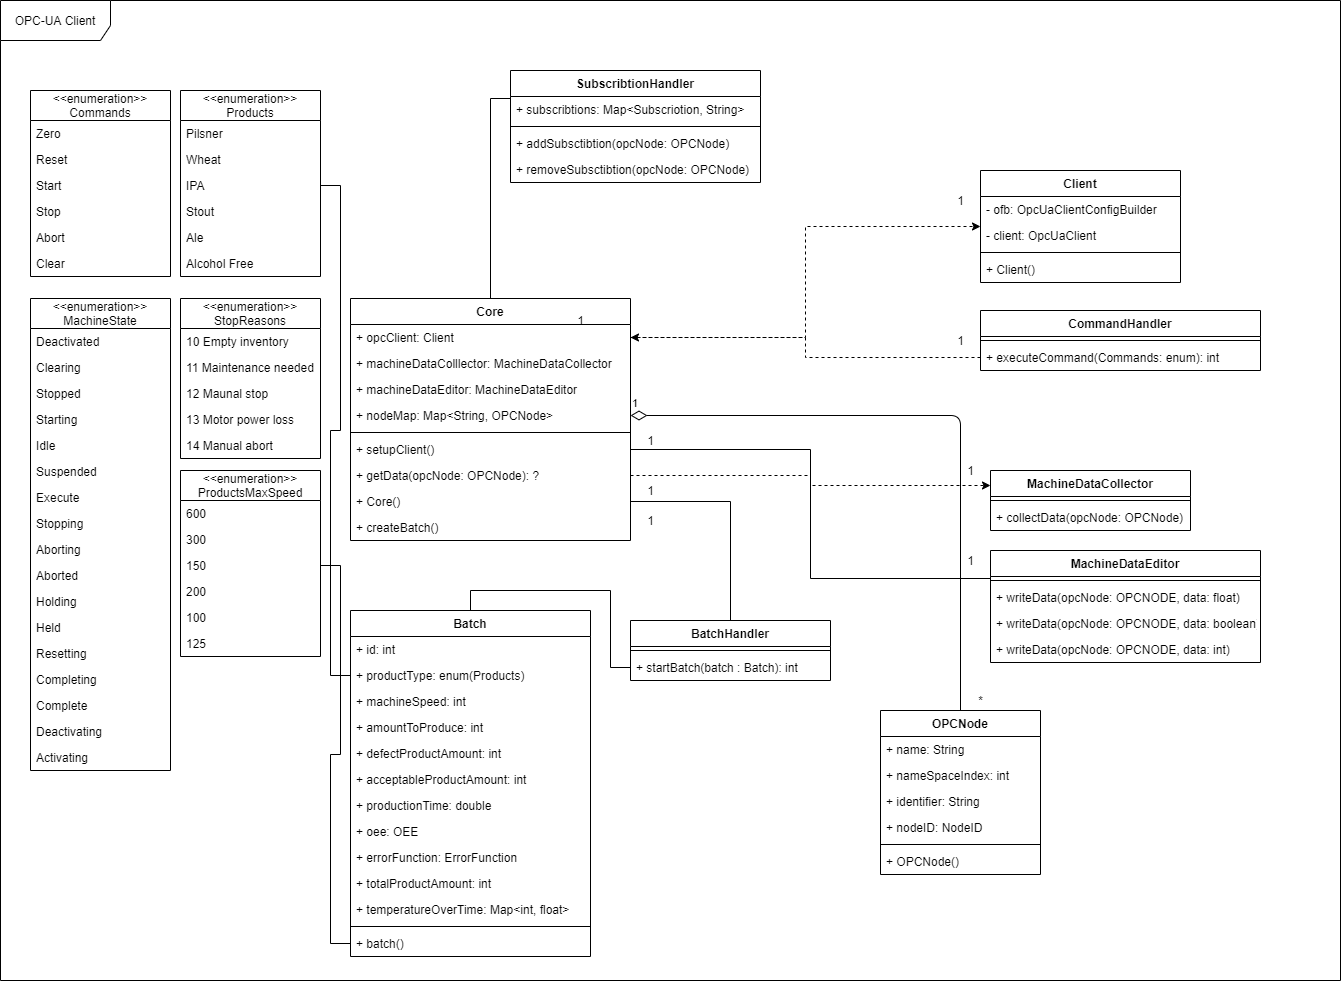
\includegraphics[scale=0.3]{images/diagrams/updated_UML_Class_Diagram.drawio.png}
\caption{Updated UML Class Diagram}
\label{figure:updated_UML_class_diagram} 
\end{figure}


The updated UML class diagram illustrates the current system idea based on the 
analysis of the system. Although this diagram only shows the 
OPC-UA client, it still gives a good idea of how this part of the system is going
to be, once implemented. \\

By using the diagram in the implementation phase, the group has a good starting 
point to expand on. The classes in the UML class diagram have a chance of not 
being implemented if the group finds them unuseful or changed to adhere to the 
program.